\documentclass[12pt]{report}
\usepackage{polski}
\usepackage[utf8]{inputenc}
\usepackage[a4paper]{geometry}
\usepackage[myheadings]{fullpage}
\usepackage{fancyhdr}
\usepackage{lastpage}
\usepackage{graphicx, wrapfig, subcaption, setspace, booktabs}
\usepackage[T1]{fontenc}
\usepackage[font=small, labelfont=bf]{caption}
\usepackage{fourier}
\usepackage[protrusion=true, expansion=true]{microtype}
\usepackage{sectsty}
\usepackage{url, lipsum}
\usepackage{tgbonum}
\usepackage{hyperref}
\usepackage{xcolor}
\usepackage{listings}
\usepackage{color}
\usepackage{float}


\definecolor{codegreen}{rgb}{0,0.6,0}
\definecolor{codegray}{rgb}{0.5,0.5,0.5}
\definecolor{codepurple}{rgb}{0.58,0,0.82}
\definecolor{backcolour}{rgb}{0.95,0.95,0.92}
 
\lstdefinestyle{mystyle}{
    backgroundcolor=\color{backcolour},   
    commentstyle=\color{codegreen},
    keywordstyle=\color{magenta},
    numberstyle=\tiny\color{codegray},
    stringstyle=\color{codepurple},
    basicstyle=\footnotesize,
    breakatwhitespace=false,         
    breaklines=true,                 
    captionpos=b,                    
    keepspaces=true,                 
    numbers=left,                    
    numbersep=5pt,                  
    showspaces=false,                
    showstringspaces=false,
    showtabs=false,                  
    tabsize=2
}

\lstset{style=mystyle}
\makeatletter

\renewcommand{\thesection}{%
  \ifnum\c@chapter<1 \@arabic\c@section
  \else \thechapter.\@arabic\c@section
  \fi
}
\makeatother
\newcommand{\code}[1]{\texttt{#1}}
\newcommand{\HRule}[1]{\rule{\linewidth}{#1}}
\onehalfspacing
\setcounter{tocdepth}{5}
\setcounter{secnumdepth}{5}
\pagestyle{fancy}  
\fancyhf{}
\chead{Sprawozdanie końcowe Java, grupa 3}
\cfoot{Strona \thepage/\pageref{LastPage}}
\graphicspath{ {images/} }
\begin{document}
{\fontfamily{cmr}\selectfont
\title{ \normalsize \textsc{}
		\\ [2.0cm]
		\HRule{0.5pt} \\
		\LARGE \textbf{{Sprawozdanie końcowe Java grupa 3}
		\HRule{0.5pt} \\ [0.5cm]
		\normalsize \today \vspace*{5\baselineskip}}
		}
}

\date{}

\author{
		Krzysztof Anderson i Michał Malinowski \\ }

\maketitle\thispagestyle{fancy}
\tableofcontents\thispagestyle{fancy}
\newpage

\sectionfont{\scshape}
\section{Wstęp teoretyczny}
Gra "Gun Game" została zbudowana w języku Java. Jest to projekt zaliczeniowy z laboratoriów przedmiotu Język i Metod Programowania 2. Pomysłodawcą jest prowadzący te zajęcia mgr inż. Paweł Zawadzki.\par
Gra dostępna jest dla dwóch graczy. Polega na zdobywaniu punktów poprzez zestrzeliwanie spadających klocków. Każdy z graczy ma do dyspozycji czołg, którym może poruszać horyzontalnie przy pomocy odpowiednich klawiszy. Podczas poruszania się gracze mogą się wzajemnie blokować, ponieważ nie ma możliwości zamiany miejsc. Do dyspozycji jest również obracająca się pod wybranym kątem wieżyczka czołgu. To dzięki niej gracze mogą decydować, w jakim kierunku zostanie oddany strzał. Każdy czołg może wystrzelić maksymalnie trzy pociski na raz i każdy kolejny dopiero, kiedy któryś z pocisków trafi w blok lub wyleci poza pole gry. \par
Podczas rozpoczęcia rozgrywki użytkownicy zostaną zapytani o nazwy graczy. Można wprowadzić własne nazwy, lub zaakceptować te wczytane z pliku konfiguracyjnego. Nazwa nie może być dłuższa niż 8 znaków.\par
W grze występują różne bloki. Każdy kolor oznacza inną ilość punktów przyznawaną za zbicie. Punkty graczy są sumowane i wyświetlane w górnej części ekranu. Celem gracza jest osiągnięcie jak największej ilości punktów. Po osiągnięciu ustalonego wcześniej progu punktowego (lub jego wielokrotności) poziom trudności gry (level) wzrasta i prędkość spadania klocków zwiększa się. \par
Dodatkowa funkcjonalność, która została wprowadzona, zakłada, że w momencie kiedy spadający klocek uderzy czołg, gracz do którego ów pojazd należał traci liczbę punktów, odpowiednią do punktów za zbicie danego koloru. \par
Gra umożliwia modyfikowanie i zapisywanie rozgrywki. Wszystko odbywa się za pomocą plików konfiguracyjnych, które tworzy program, lub które możemy sami stworzyć według odpowiedniego wzorca. Program jest zabezpieczony przed wprowadzaniem błędnych danych.



\section{Osiągnięte cele}
Program spełnia wszystkie wymagania, jakie zostały postawione przed tym projektem. Program:
\begin{itemize}
    \item wczytuje plik konfiguracyjny określający podstawowe parametry programu;
    \item umożliwia ustawienie nazw obu graczy;
    \item umożliwia użytkownikowi sterowanie obydwoma czołgami, tj. przesuwać je na boki, obracać ich lufy oraz strzelać;
    \item każdorazowo po zdobyciu odpowiedniej liczby punktów ustalonej przez plik konfiguracyjny zwiększa poziom trudności przyspieszając spadające klocki;
    \item czołgi nie mogą zamienić się miejscami, ani przenikać;
    \item zapisuje plik obecnej rozgrywki, który można następnie wczytać;
    \item obsługuje błędy związane z podaniem niepoprawnego pliku konfiguracyjnego.
\end{itemize}
Ponadto zostały dodane dodatkowe funkcjonalności. Program:
\begin{itemize}
    \item pozwala na ustawienie wybranej przez użytkownika liczby rodzajów klocków, dowolnych kolorów tych obiektów (używając do tego parametrów RGB) oraz punktów za ich zbicie (każdy kolor, to możliwa inna liczba punktów.
    \item wprowadza utrudnienie, polegające na punktach ujemnych za kolizję czołgów z klockami. Graczowi, na którego czołg wpada klocek, jest odejmowana liczba punktów odpowiednia dla danego typu klocka.
    \item pozwala ustawić maksymalną wysokość i szerokość generowanych klocków.
    \item blokuje nadmierną liczbę pocisków wystrzelonych przez graczy. Na planszy gry mogą znajdować się jedynie trzy pociski każdego gracza. Możliwość wystrzelenia kolejnego pocisku pojawia się, kiedy jeden z pocisków zbije klocek lub wyleci poza planszę.
    \item ogranicza kąt obrotu lufy, w zależności od podanego parametru w pliku konfiguracyjnym.
    
\end{itemize}


\section{Co zostało zmienione względem specyfikacji}
    
    \subsection{GUI}
      Zmieniona została stylistyka programu, z domyślnej (szarej), na połączenie czerni i bieli w elementach interfejsu użytkownika oraz ciemnej szarości na planszy rozgrywki. Dodany został do okna rozgrywki panel "Level", wskazujący na aktualny poziom rozgrywki począwszy od zera.
      
     \subsection{Inserter}
     Klasa \code{Inserter} rozszerza \code{Thread}, zamiast implementować \code{Runnable}.
     Klasa otrzymała również dwa nowe pola: \code{speed} oraz \code{running}. Pierwsze ustala prędkość spadania generowanych klocków, a druga decyduje, czy nowe klocki mają się pojawiać.
     
     \subsection{Board}
     Zrezygnowaliśmy z obsługi automatycznych ruchów wątkiem \code{Cycle}, na rzecz znajdującego się w bibliotece \code{Swing} \code{Timer}-a.
     Klasa \code{Board} posiada nowe pola:
     \begin{itemize}
         \item przechowujące przyciski sterujące grą;
         \item \code{File config} przechowujące wczytany plik konfiguracyjny;
         \item \code{playerLeft} i \code{playerRight} zamiast \code{player1} i \code{player2};
         \item \code{background} przechowujące tło planszy;
         \item \code{level} przechowujące poziom trudności rozgrywki;
         \item \code{threshold} przechowujące liczbę punktów po której poziom się zwiększa;
         \item \code{maxWidth} oraz \code{maxHeight} przechowujące maksymalne rozmiary klocków;
         \item \code{blockColors} oraz \code{blockPoints} przechowujące kolory bloków i odpowiadające im punkty;
         \item \code{writer} przechowujące obiekt klasy \code{Writer} który zapisuje stan rozgrywki.
     \end{itemize}
     Klasa otrzymała również nowe metody:
     \begin{itemize}
         \item \code{read}, która czyta plik konfiguracyjny;
         \item \code{reset}, która pozbywa się wszystkich obiektów z planszy;
         \item \code{clean}, która usuwa niewidoczne już elementy;
         \item \code{paintComponent} oraz \code{doDrawing}, które odpowiadają za wyświetlanie elementów gry na planszy;
         \item \code{updateMissiles, updateBlocks, updateTanks} oraz \code{checkCollisions}, które miały znajodwać się w nieistniejącej klasie \code{Cycle}.
     \end{itemize}
     
     \subsection{Sprite}
     Klasa ta, otrzymała nową metodę \code{getBounds} zwracającą wymiary i położenie prostokąta otaczającego dany obiekt, potrzebnego do sprawdzania kolizji.
     
     \subsection{Block}
     Klocki nie są ustalonymi kształtami, tylko losowo generowanymi prostokątami. Klasa \code{Block} nie jest więc rozszerzana. Prędkość spadania nie zwiększa się o~1, tylko o 0.25 i jej pole \code{dy} jest typu \code{double} a nie \code{int}. Maksymalna prędkość spadania została ograniczona do 100, ponieważ większe wartości, uniemożliwiłyby poprawną rozgrywkę. \code{Block} posiada nową metodę \code{getRandomNumber}, która generuje losową liczbę. Dodatkowo, klocki nie znikają po dotarciu na linię czołgów, jednak dopiero wtedy, kiedy przekroczą granicę \code{board}-a.
     
     \subsection{Body oraz Gun}
     Metody \code{move} z tych dwóch klas oraz metoda \code{drawGun} z klasy \code{Gun} zostały przeniesione do klasy, \code{Player}.
     
     \subsection{Player}
     Klasa ta otrzymała nowe pola:
     \begin{itemize}
         \item \code{da} wyznaczające przyrost kąta obrotu lufy;
         \item \code{maxGunAngle} wyznaczające maksymalny kąt obrotu lufy;
         \item \code{keyMoveLeft}, \code{keyMoveRight}, \code{keyTurnLeft}, \code{keyTurnRight}, \code{keyFire}, zawierające przyciski, przy pomocy których możliwe jest sterowanie czołgiem;
         \item \code{missiles}, które jest listą pocisków wystrzelonych przez danego gracza.
     \end{itemize}
        Metoda \code{draw}, jest przeniesioną z klasy \code{Gun} metodą, służącą do rysowania obracającej się lufy czołgu. Nazwy graczy nie są sprawdzane pod kątem polskich znaków i spacji. Jedynym ograniczeniem jest długość nazwy do 8 znaków.
        
    \subsection{Reader}
    Pozwalamy na podanie ujemnej liczby punktów graczy. Klasa ta posiada dodatkowo pola:
    \begin{itemize}
        \item \code{inputScanner} służącą do wczytywania linii z pliku konfiguracyjnego;
        \item \code{inserter} będącą referencją do obiektu \code{inserter} utworzonego w obiekcie \code{board};
        \item \code{board} będącą referencją do głównego obiektu \code{board}.
    \end{itemize}
    Zmienione i dodane metody to:
    \begin{itemize}
        \item \code{readFile} nie posiada argumentu wywołania;
        \item \code{trimString} polegająca na pomijaniu komentarzy z pliku, oraz na usuwaniu zbędnych białych znaków.
    \end{itemize}
    
    \subsection{Writer}
    W tej klasie zrezygnowano z pola \code{File file}, gdyż była ono niepotrzebne. Metoda \code{writeFile} dynamicznie dostosowuje się do liczby różnych kolorów i punktów klocków, tworząc czytelny, z odpowiednimi komentarzami, plik konfiguracyjny w pełni poprawny do ponownego wczytania, jako stan początkowy gry.
        
    \subsection{Nowe klasy}
    Powstała jedna nowa klasa, \code{MyCustomFilter}, która filtruje pliki widoczne przy wybieraniu pliku konfiguracyjnego. Dzięki niej widać tylko foldery i pliki tekstowe.
    \subsection{Czego brakuje}
    Jedyną brakującą rzeczą jest \code{executable jar}, którego nie utworzyliśmy.

\section{Przykłady uruchomienia}
W tym rozdziale zaprezentowane zostaną przykłady uruchomienia programu.

\begin{itemize}
    \begin{figure}[H]
    \centering
    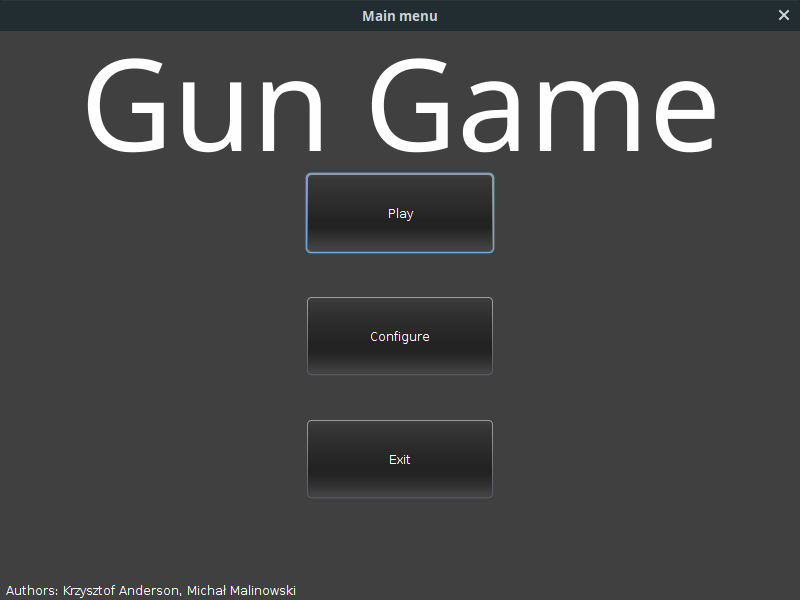
\includegraphics[width=14cm]{obrazy/mainMenu.png}
    \caption{Główne menu}
    \label{main menu screen}
    \end{figure}
    \item Ekran głównego menu w nowej stylistyce.
    \begin{figure}[H]
    \centering
    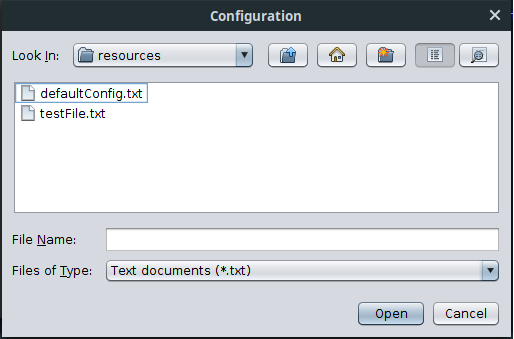
\includegraphics[width=14cm]{obrazy/fileChooser.png}
    \caption{Wybór konfiguracji}
    \label{file chooser}
    \end{figure}
    \item Ekran wyboru pliku konfiguracyjnego. Widoczne są jedynie fodlery i pliki tekstowe.
    \begin{figure}[H]
    \centering
    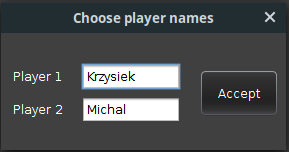
\includegraphics[width=14cm]{obrazy/playerName.png}
    \caption{Ekran wyboru imion}
    \label{name choice screen}
    \item Ekran służący do podania imion graczy. Imiona nie mogą przekroczyć 8 znaków
    \end{figure}
    \begin{figure}[H]
    \centering
    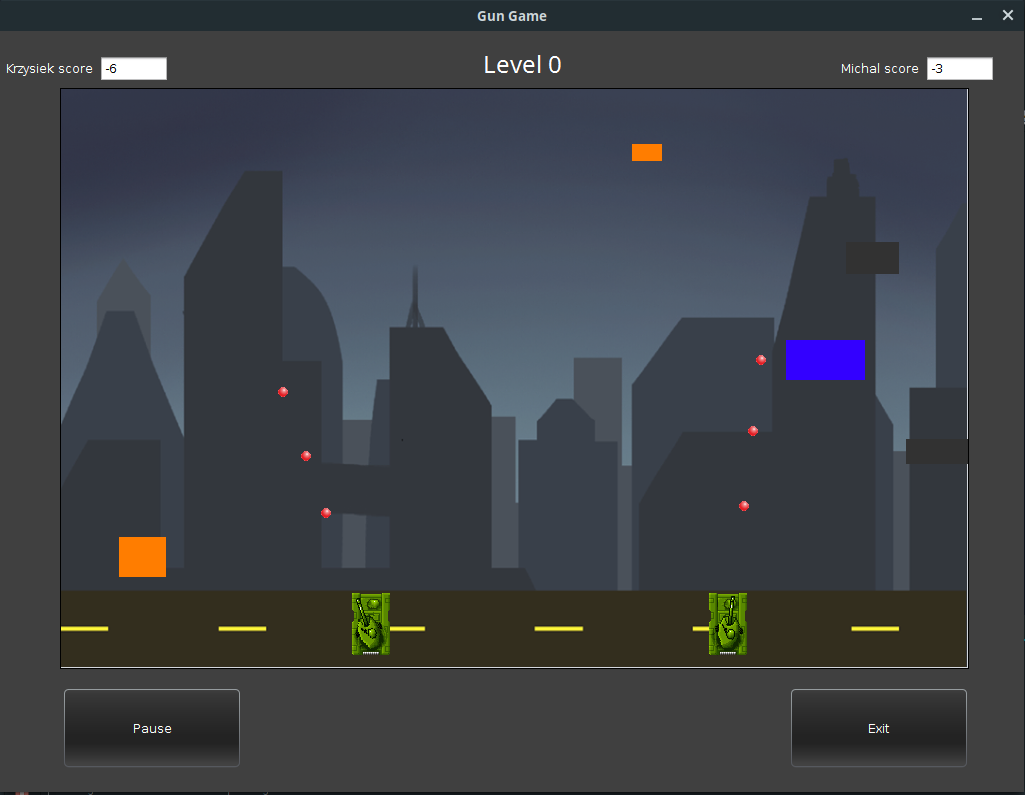
\includegraphics[width=14cm]{obrazy/screenGame.png}
    \caption{Ekran gry}
    \label{game screen}
    \end{figure}
    \item Ekran rozgrywki, widzimy spadające klocki, czołgi z obróconymi lufami oraz wystrzelone przez nie pociski.
    \begin{figure}[H]
    \centering
    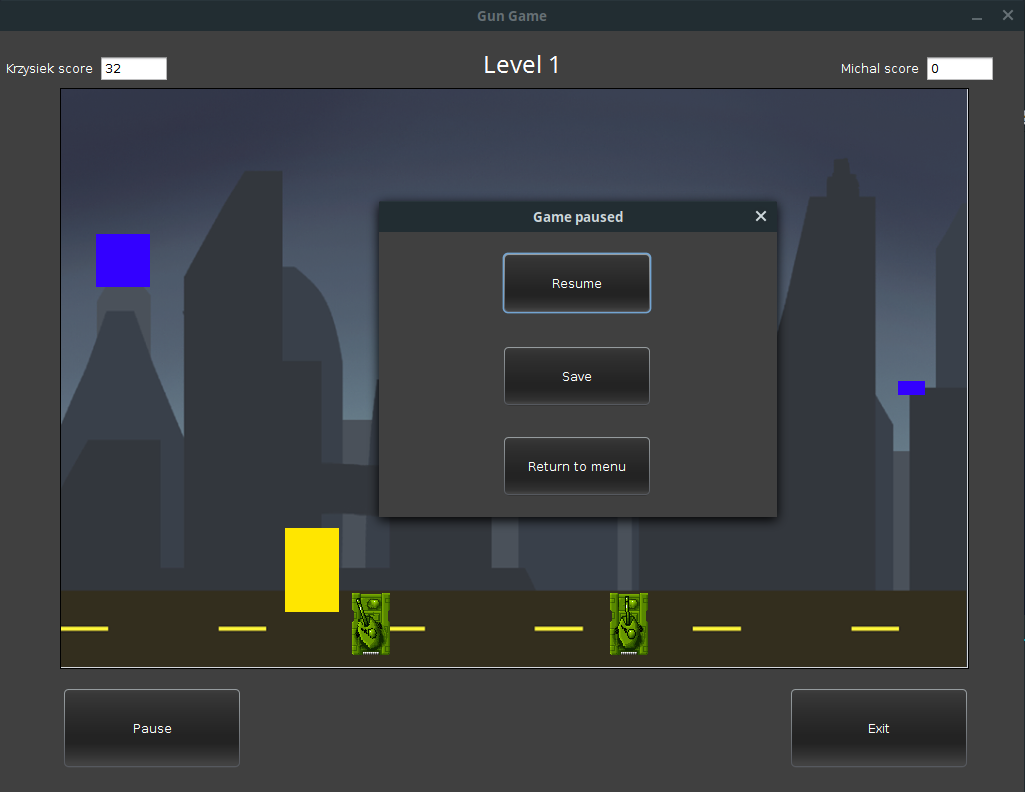
\includegraphics[width=14cm]{obrazy/pauseMenu.png}
    \caption{Ekran pauzy}
    \label{pause screen}
    \end{figure}
    \item Zatrzymana rozgrywka, razem z oknem pauzy. Z tego poziomu możemy wznowić rozgrywkę, zapisać ją, lub też wrócić do menu głównego.
\end{itemize}



\section{Testowanie}
Testy programu zostały podzielone na dwie kategorie.

\subsection{Testy jednostkowe}
Do testów jednostkowych zostało wykorzystane narzędzie JUnit.
\begin{itemize}
    \item \code{testCheckCollisions} w znanej lokalizacji zostaje zainicjowany blok i gracz. Do listy pocisków gracza zostaje dodany nowy pocisk, a następnie zostaje wywołania metoda \code{checkCollisions}. Spodziewamy się, że kolizja pocisku i bloku zostanie wykryta i liczba punktów gracza wzrośnie. Zapisujemy stary stan punktów i porównujemy z nowym. Jeżeli wyniki się różnią, test przechodzi pozytywnie.
    \item \code{testGetImageDimensions} zostaje wprowadzony obrazek o znanych wymiarach (10x10). Spodziewamy się, że testowana metoda zwróci dokładnie taką wartość. W przeciwnym wypadku test kończy się niepowodzeniem.
    \item \code{testGetRandomNumber} wprowadzony jest zakres od 0 do 10, w którym ma zostać wylosowana liczba. Po każdym losowaniu sprawdzane jest czy wylosowana liczba jest z danego zakresu. Test jest przeprowadzany 10 razy, aby kilkukrotnie wylosować nową liczbę i poddać ją badaniu. Kiedy program napotka na liczbę spoza zakresu, zapali flagę \code{successFlag} na \code{false} i test nie przejdzie pozytywnie.
    \item \code{testTrimLine} zostaje wprowadzony do metody \code{trimLine} znany plik, który zawiera zakomentowany tekst. Spodziewamy się, że metoda \code{trimLine} usunie zbędne białe znaki i pominie zakomentowany wiersz. Jeżeli metoda działa poprawnie, powinna zapisać do czterech kolejnych zmiennych pierwszą, drugą, trzecią i piątą linię. W momencie kiedy zmienne zgadzają się ze wzorcem, test przechodzi pozytywnie.
    \item \code{testFire} zostaje zainicjowany gracz. Zostaje dla niego wywołana metoda \code{fire}. Spodziewamy się, że po oddaniu strzału, lista pocisków danego gracza zwiększy się. Porównujemy stary rozmiar listy z nowym. Jeżeli wyniki się różnią, test przechodzi pozytywnie.
\end{itemize}

\subsection{Testy akceptacyjne ręczne}
Program jest w stanie poprawnie obsłużyć błędne dane.
    \begin{figure}[H]
    \centering
    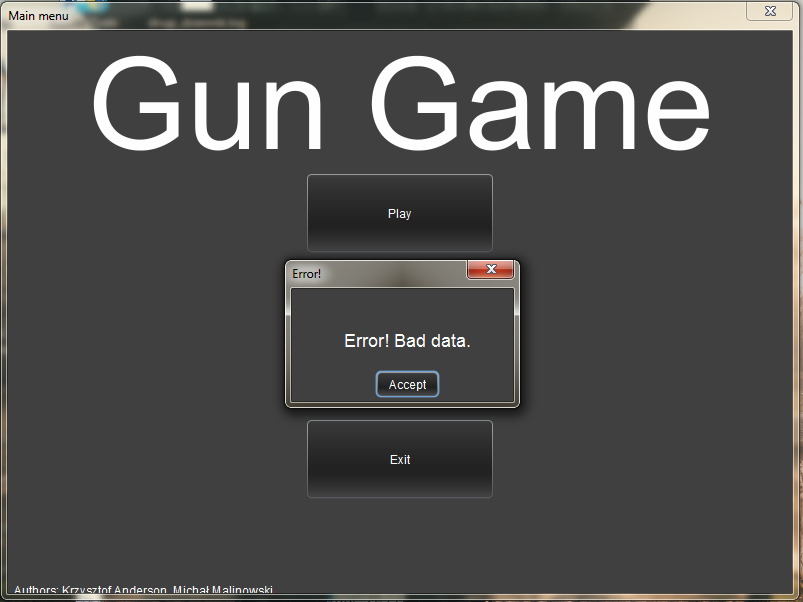
\includegraphics[width=14cm]{obrazy/configBadData.png}
    \caption{Błędny plik konfiguracyjny}
    \label{config bad data}
    \end{figure}
    \begin{figure}[H]
    \centering
    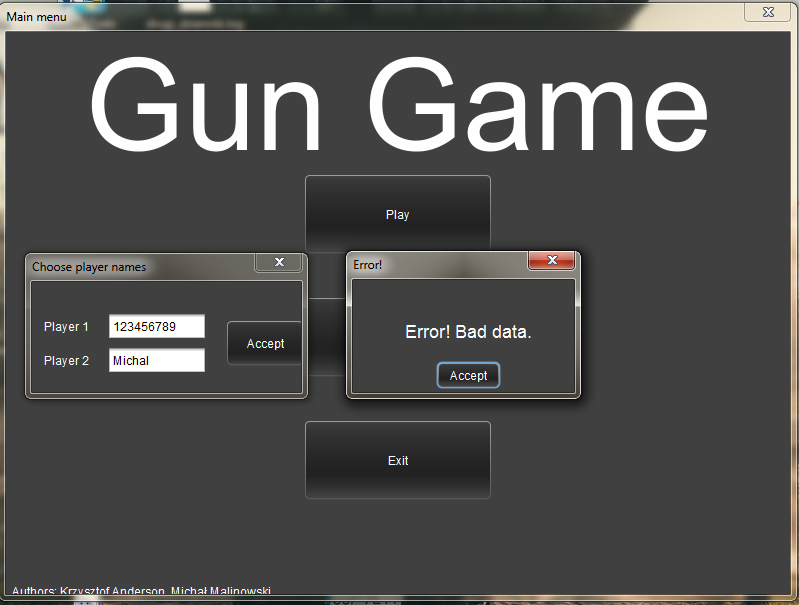
\includegraphics[width=14cm]{obrazy/nameBadData.png}
    \caption{Błędna nazwa gracza}
    \label{bad player name}
    \end{figure}
    \newpage
    Nie da się również zmieniać rozmiarów okna.
    \begin{figure}[H]
    \centering
    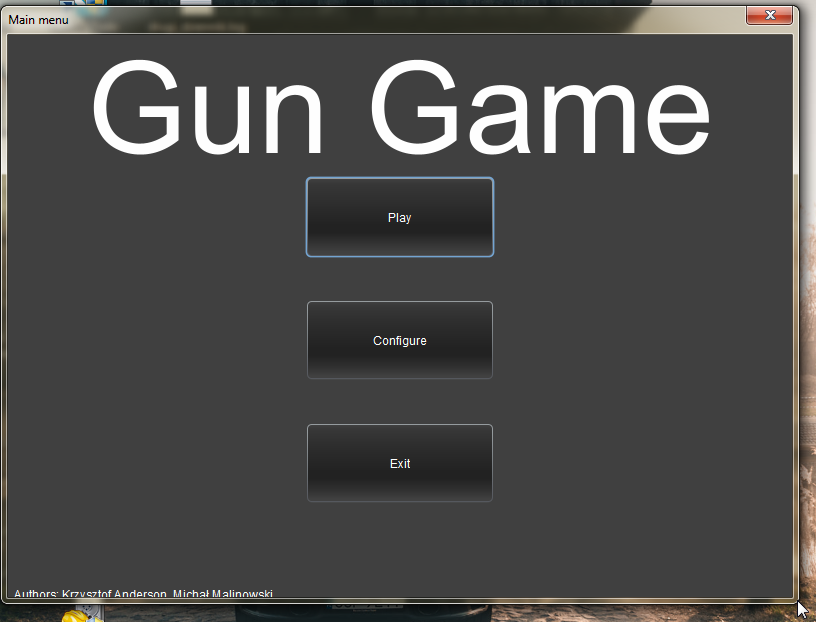
\includegraphics[width=14cm]{obrazy/resizable.png}
    \caption{Okno nie jest rozszerzalne}
    \label{not resizable}
    \end{figure}
\end{document}